\documentclass[border=10pt]{standalone}
\usepackage{tikz}\usepackage{amsmath}\usetikzlibrary{arrows.meta}
\begin{document}
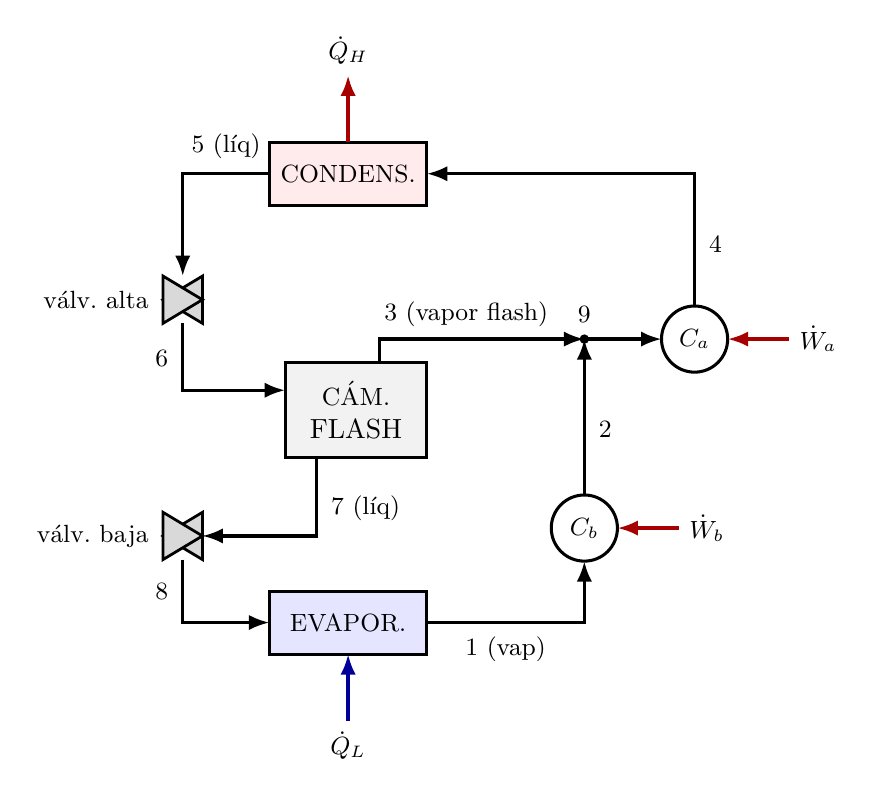
\begin{tikzpicture}[line width=1pt,>={Latex[length=2.6mm]}]
  % ===================== componentes =====================
  % condensador (arriba)
  \fill[red!8] (2.0,5.4) rectangle (4.0,6.2); \draw[line width=1.1pt] (2.0,5.4) rectangle (4.0,6.2);
  \node at (3.0,5.8){\small CONDENS.};
  % camara flash (economizador)
  \fill[black!5] (2.2,2.2) rectangle (4.0,3.4); \draw[line width=1.1pt] (2.2,2.2) rectangle (4.0,3.4);
  \node[align=center] at (3.1,2.8){\small CÁM.\\FLASH};
  % evaporador (abajo)
  \fill[blue!10] (2.0,-0.3) rectangle (4.0,0.5); \draw[line width=1.1pt] (2.0,-0.3) rectangle (4.0,0.5);
  \node at (3.0,0.1){\small EVAPOR.};
  % compresor de baja
  \draw[line width=1.1pt] (6.0,1.3) circle (0.42); \node at (6.0,1.3){\small $C_{b}$};
  % compresor de alta
  \draw[line width=1.1pt] (7.4,3.7) circle (0.42); \node at (7.4,3.7){\small $C_{a}$};
  % valvula alta
  \fill[black!15] (0.65,4.2)--(1.15,4.5)--(1.15,3.9)--cycle; \draw[line width=1.0pt] (0.65,4.2)--(1.15,4.5)--(1.15,3.9)--cycle;
  \fill[black!15] (1.15,4.2)--(0.65,4.5)--(0.65,3.9)--cycle; \draw[line width=1.0pt] (1.15,4.2)--(0.65,4.5)--(0.65,3.9)--cycle;
  \node[left] at (0.6,4.2){\small válv.\ alta};
  % valvula baja
  \fill[black!15] (0.65,1.2)--(1.15,1.5)--(1.15,0.9)--cycle; \draw[line width=1.0pt] (0.65,1.2)--(1.15,1.5)--(1.15,0.9)--cycle;
  \fill[black!15] (1.15,1.2)--(0.65,1.5)--(0.65,0.9)--cycle; \draw[line width=1.0pt] (1.15,1.2)--(0.65,1.5)--(0.65,0.9)--cycle;
  \node[left] at (0.6,1.2){\small válv.\ baja};
  % ===================== tuberias =====================
  % evap -> compresor baja
  \draw[->,line width=1.2pt] (4.0,0.1)--(6.0,0.1)--(6.0,0.88); \node[below] at (5.0,0.05){\small 1 (vap)};
  % compresor baja -> nodo de mezcla 9
  \draw[->,line width=1.2pt] (6.0,1.72)--(6.0,3.7); \node[right] at (6.05,2.55){\small 2};
  % vapor flash 3 -> nodo de mezcla 9
  \draw[->,line width=1.2pt] (3.4,3.4)--(3.4,3.7)--(6.0,3.7); \node[above] at (4.5,3.72){\small 3 (vapor flash)};
  \fill (6.0,3.7) circle (0.06); \node[above] at (6.0,3.78){\small 9};
  % nodo 9 -> compresor alta
  \draw[->,line width=1.2pt] (6.0,3.7)--(6.98,3.7);
  % compresor alta -> condensador
  \draw[->,line width=1.2pt] (7.4,4.12)--(7.4,5.8)--(4.0,5.8); \node[right] at (7.45,4.9){\small 4};
  % condensador -> valvula alta
  \draw[->,line width=1.2pt] (2.0,5.8)--(0.9,5.8)--(0.9,4.5); \node[above] at (1.45,5.85){\small 5 (líq)};
  % valvula alta -> camara flash
  \draw[->,line width=1.2pt] (0.9,3.9)--(0.9,3.05)--(2.2,3.05); \node[left] at (0.85,3.45){\small 6};
  % camara flash (liquido) -> valvula baja
  \draw[->,line width=1.2pt] (2.6,2.2)--(2.6,1.2)--(1.15,1.2); \node[right] at (2.65,1.55){\small 7 (líq)};
  % valvula baja -> evaporador
  \draw[->,line width=1.2pt] (0.9,0.9)--(0.9,0.1)--(2.0,0.1); \node[left] at (0.85,0.5){\small 8};
  % ===================== interacciones =====================
  \draw[->,red!65!black,line width=1.3pt] (3.0,6.2)--(3.0,7.05); \node[above] at (3.0,7.05){\small $\dot Q_H$};
  \draw[->,blue!60!black,line width=1.3pt] (3.0,-1.15)--(3.0,-0.3); \node[below] at (3.0,-1.15){\small $\dot Q_L$};
  \draw[<-,red!65!black,line width=1.3pt] (6.42,1.3)--(7.2,1.3); \node[right] at (7.2,1.3){\small $\dot W_b$};
  \draw[<-,red!65!black,line width=1.3pt] (7.82,3.7)--(8.6,3.7); \node[right] at (8.6,3.7){\small $\dot W_a$};
\end{tikzpicture}
\end{document}
